\documentclass[a4paper,12pt]{article}
\usepackage{amsmath, amsthm, amssymb}
\usepackage{pgf,tikz} % 添加绘图
\usetikzlibrary{positioning}
\usepackage{tabularx}
\usepackage{enumitem}
\usepackage{fancyref}

\usepackage[top=1in,bottom=1in,left=1in,right=1in]{geometry} % 用于设置页面布局
\usepackage{xeCJK} % 用于使用本地字体
\usepackage[super, square, sort&compress]{natbib} % 处理参考文献
\usepackage{titlesec, titletoc} % 设置章节标题及页眉页脚
%\usepackage{xCJKnumb} % 中英文数字转换
\usepackage{amssymb}
\usepackage{amsmath} % 在公式中用\text{文本}输入中文
\usepackage{diagbox}
\usepackage{multirow} % 表格中使用多行
\usepackage{booktabs} % 表格中使用\toprule等命令
\usepackage{rotating} % 使用sidewaystable环境旋转表格
\usepackage{tabularx}
\usepackage{graphicx} % 处理图片
\usepackage{footnote} % 增强的脚注功能,可添加表格脚注
\usepackage{threeparttable} % 添加真正的表格脚注,示例见README
\usepackage{hyperref} % 添加pdf书签

\usepackage{tikz}
\usetikzlibrary{shapes,arrows,shadows}

% 字体设置
\setmainfont{Times New Roman}
\setsansfont[Scale=MatchLowercase,Mapping=tex-text]{PT Sans}
\setmonofont[Scale=MatchLowercase]{PT Mono}
\setCJKmainfont[ItalicFont={Kaiti SC}, BoldFont={Heiti SC}]{Songti SC}
\setCJKsansfont{Heiti SC}
\setCJKmonofont{Songti SC}
% \setCJKmainfont[BoldFont={FZXiaoBiaoSong-B05S}]{Songti SC}
% \setCJKfamilyfont{kai}[BoldFont=Heiti SC]{Kaiti SC}
% \setCJKfamilyfont{song}[BoldFont=Heiti SC]{Songti SC}
% \setCJKfamilyfont{hei}[BoldFont=Heiti SC]{Heiti SC}
% \setCJKfamilyfont{fsong}[BoldFont=Heiti SC]{Songti SC}
% \newcommand{\kai}[1]{{\CJKfamily{kai}#1}}
% \newcommand{\hei}[1]{{\CJKfamily{hei}#1}}
% \setromanfont[Mapping=tex-text]{TeXGyrePagella}
% \setsansfont[Scale=MatchLowercase,Mapping=tex-text]{TeXGyrePagella}
% \setmonofont[Scale=MatchLowercase]{Courier New}
%%设置常用中文字号,方便调用
\newcommand{\erhao}{\fontsize{22pt}{\baselineskip}\selectfont}
\newcommand{\xiaoerhao}{\fontsize{18pt}{\baselineskip}\selectfont}
\newcommand{\sanhao}{\fontsize{16pt}{\baselineskip}\selectfont}
\newcommand{\xiaosanhao}{\fontsize{15pt}{\baselineskip}\selectfont}
\newcommand{\sihao}{\fontsize{14pt}{\baselineskip}\selectfont}
\newcommand{\xiaosihao}{\fontsize{12pt}{\baselineskip}\selectfont}
\newcommand{\wuhao}{\fontsize{10.5pt}{\baselineskip}\selectfont}
\newcommand{\xiaowuhao}{\fontsize{9pt}{\baselineskip}\selectfont}
\newcommand{\liuhao}{\fontsize{7.5pt}{\baselineskip}\selectfont}

% 章节标题显示方式及页眉页脚设置
% \item xCJKnumb是自己额外安装的包
% \item titleformat命令定义标题的形式
% \item titlespacing定义标题距左、上、下的距离
\titleformat{\section}{\raggedright\large\bfseries}{\thesection}{1em}{}
\titleformat{\subsection}{\raggedright\normalsize\bfseries}{\thesubsection}{1em}{}
\titlespacing{\section}{0pt}{*0}{*2}
\titlespacing{\subsection}{0pt}{*0}{*1}
% 由于默认的2em缩进不够,所以我手动调整了,但是在windows下似乎2.2就差不多了,或者是article中没有这个问题
\setlength{\parindent}{2.2em}

% 设置表格标题前后间距
\setlength{\abovecaptionskip}{0pt}
\setlength{\belowcaptionskip}{0pt}


\renewcommand{\refname}{\bfseries{参~考~文~献}} %将Reference改为参考文献(用于 article)
% \renewcommand{\bibname}{参~考~文~献} %将bibiography改为参考文献(用于 book)
\renewcommand{\baselinestretch}{1.38} %设置行间距
\renewcommand{\figurename}{\small\ttfamily 图}
\renewcommand{\tablename}{\small\ttfamily 表}

\setlength{\parindent}{0em}
\setlength{\parskip}{0.5em}

\newtheorem{definition}{定义}
\newtheorem{lemma}{引理}
\newtheorem{proposition}{命题}
\newtheorem{program}{程序}
\newtheorem{convention}{约定}
\renewcommand*{\proofname}{证明}

\title{关于前传与反传的笔记}
\author{苑明理}
\date{2018年12月}

\begin{document}

\maketitle{}

\renewcommand\contentsname{目录}
\setcounter{tocdepth}{2}
\tableofcontents

\newpage

\section{示例}

\subsection{平流方程}

$$
\frac{\partial N}{\partial t} = - u \frac{\partial N}{\partial x}
$$

$$
N_i^{+} = N_i - \frac{u \tau }{2 \lambda}(N_{i+1} - N_{i-1})
$$

\begin{figure}[ht]
\centering
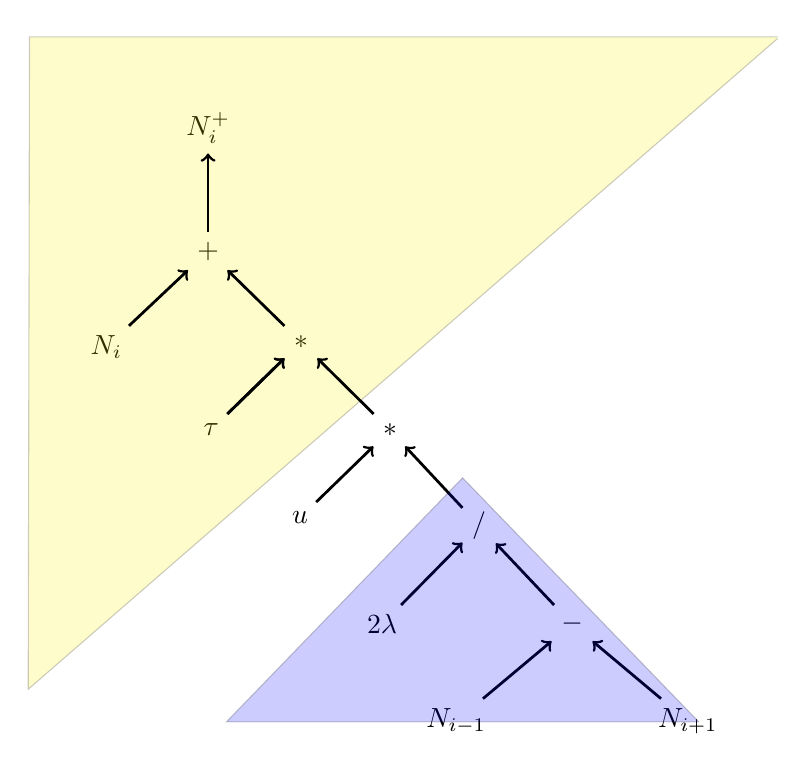
\begin{tikzpicture}
% nodes %

\node[text centered] (p0) {};
\node[below left = 1 of p0, text centered] (f) {$N_i^{+}$};
\node[below = 1 of f, text centered] (plus) {$+$};
\node[below left = 1 of plus, text centered] (c) {$N_i$};
\node[below right = 1 of plus, text centered] (multi) {$*$};
\node[below left = 1 of multi, text centered] (tau) {$\tau$};
\node[below right = 1 of multi, text centered] (multi1) {$*$};
\node[below left = 1 of multi1, text centered] (u) {$u$};
\node[below right = 1 of multi1, text centered] (divid) {$/$};
\node[below left = 1 of divid, text centered] (ratio) {$2 \lambda$};
\node[below right = 1 of divid, text centered] (minus) {$-$};
\node[below left = 1 of minus, text centered] (p) {$N_{i-1}$};
\node[below right = 1 of minus, text centered] (n) {$N_{i+1}$};

% edges %
\draw[fill=yellow, opacity=0.2]  (6.0, 0) -- (0:-3.5) -- (-113:9.0) -- (-0.2:6.0);
\draw[->, line width= 1] (plus) -- (f);
\draw[->, line width= 1] (c) -- (plus);
\draw[->, line width= 1] (multi) -- (plus);
\draw[->, line width= 1] (tau) -- (multi);
\draw[->, line width= 1] (tau) -- (multi);
\draw[->, line width= 1] (multi1) -- (multi);
\draw[->, line width= 1] (u) -- (multi1);
\draw[->, line width= 1] (divid) -- (multi1);
\draw[->, line width= 1] (ratio) -- (divid);
\draw[->, line width= 1] (minus) -- (divid);
\draw[->, line width= 1] (p) -- (minus);
\draw[->, line width= 1] (n) -- (minus);
\draw[fill=blue, opacity=0.2]  (5.0, -8.7) -- (-1.0, -8.7) -- (2.0, -5.6) -- (5.0, -8.7);

\end{tikzpicture}
\caption{表达式树}
\end{figure}

\newpage

\subsection{扩散方程}


\newpage

\end{document}
